Zum Vergleich  mit den  soeben dimensionierten PI-  und PID-Reglern  sind hier
noch  die Resultate  der  Dimensionierung mittels  unseres Tools  gezeigt. Wie
zu  erwarten   weisen  die   Resultate  der  Faustformeln   keine  gr\"osseren
Abweichenungen  zu  Tabelle~\ref{tab:ff_results}  auf.

Es  ist  aber  klar  zu  erkennen,  dass  die  mittels  der  Phasengangmethode
berechneten  Reglerwerte   teilweise  deutlich  von  den   manuell  bestimmten
Zahlen  abweichen. Der  Grund daf\"ur  liegt  in  den Optimierungen,  die  das
Tool  zus\"atzlich zu  den  in diesem  Abschnitt  gezeigten Berechnungen  noch
ausf\"uhrt (siehe dazu auch Abschnitt~\ref{sec:software}).

\todo{Bild PI-Regler}
\todo{Bild PID-Regler}

%\begin{figure}[h!, width=\pagewidth]
%    \centering
%    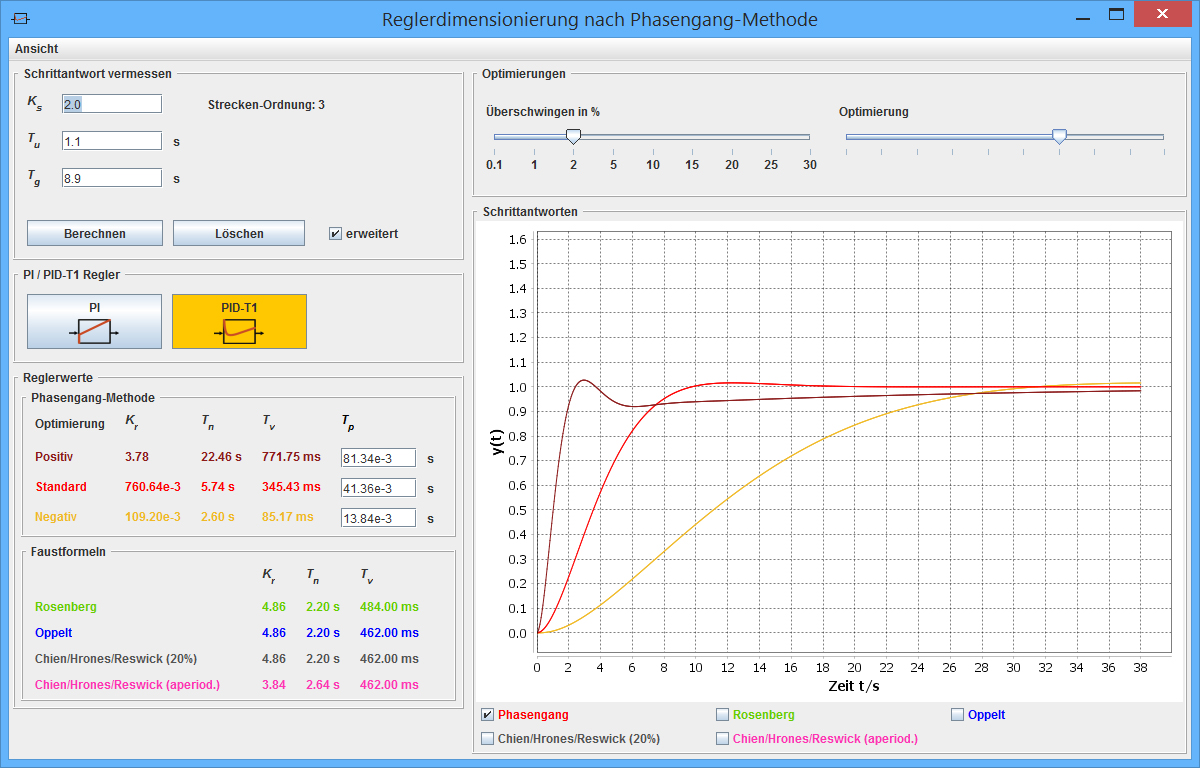
\includegraphics[width=\textwidth]{images/tool2UeberschwingenOptimierungPID.jpg}
%    \caption{Plots der Schrittantworten nach Phasengangmethode, PID-Regler, 2\% \"Uberschwingen}
%    \label{fig:tool2UberschwingenPID}
%\end{figure}
%
%\begin{figure}[h!, width=\pagewidth]
%    \centering
%    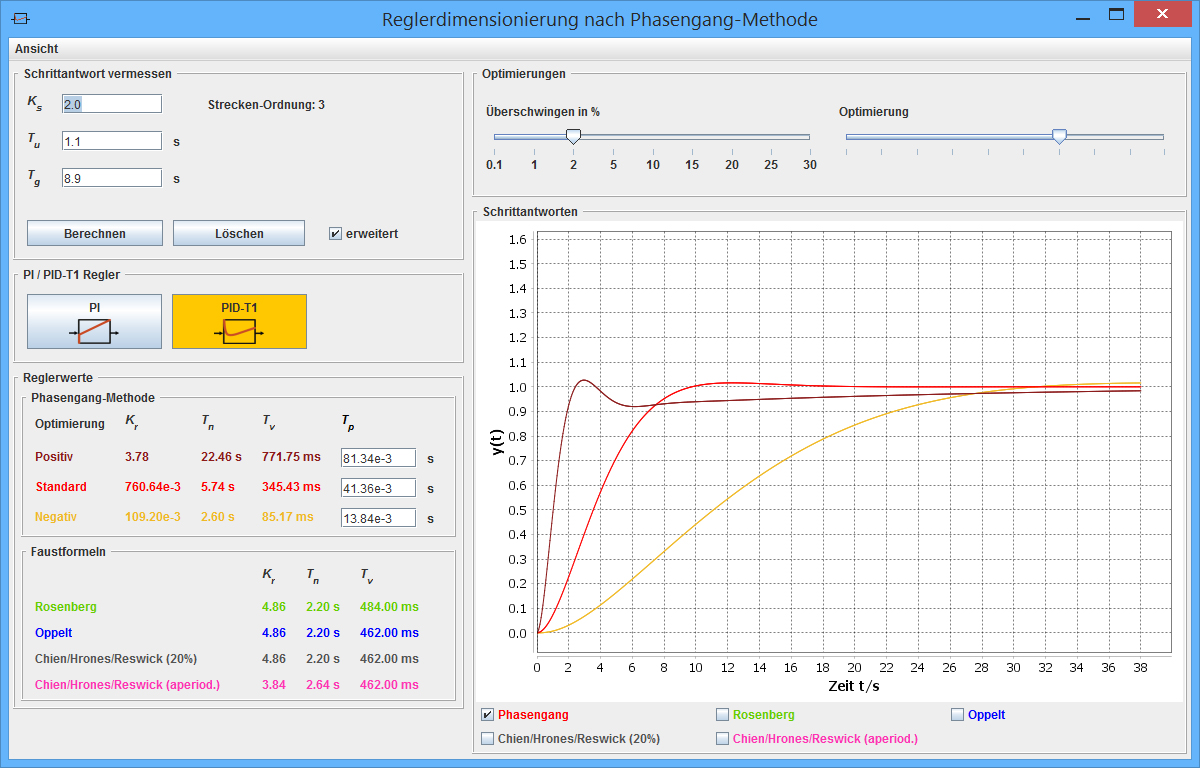
\includegraphics[width=\textwidth]{images/tool2UeberschwingenOptimierungPID.jpg}
%    \caption{Plots der Schrittantworten nach Phasengangmethode, PID-Regler, 2\% \"Uberschwingen}
%    \label{fig:tool2UberschwingenPID}
%\end{figure}
